\documentclass{article}
\newlength{\sliceheight}\setlength{\sliceheight}{3.5cm}
\usepackage{subcaption,graphicx,calc,tabu,xcolor,mathtools,listings,matlab-prettifier,mdframed,setspace}
\usepackage[margin=2cm]{geometry}
\graphicspath{{figs/}}
\newcommand{\matlabdir}{C:/Users/Jesse/Documents/m/Research/wmlseg/workspace/}
\newenvironment{subfigureside}[1][\sliceheight]{\begin{subfigure}{\textwidth}\centering\parbox[b][#1-1em][c]{0.5cm}{\subcaption{}} }{\end{subfigure}}
\newenvironment{subfiguretop}[1][\sliceheight]{\begin{minipage}{#1}\begin{subfigure}{\textwidth}\centering\subcaption{}}{\end{subfigure}\end{minipage}}
\newcommand{\matlabsty}{\color{black}\ttfamily\footnotesize}
\global\mdfdefinestyle{graybar}{topline=false,rightline=false,bottomline=false,linewidth=0.2em,linecolor=lightgray,innertopmargin=0pt,innerbottommargin=0pt}
\lstnewenvironment{matlab}{\linespread{1}\mdframed[style=graybar]\lstset{style=Matlab-editor,basicstyle=\matlabsty,basewidth=0.5em}}{\endmdframed}
\newcommand{\includecode}[1]{\subsubsection{\ttfamily{#1}}
  \begin{mdframed}[style=graybar]\lstinputlisting[style=Matlab-editor,basicstyle=\linespread{1}\matlabsty]{\matlabdir#1}\end{mdframed}}
\renewcommand{\b}{\beta}
\begin{document}
  \begin{doublespace}
%  \begin{figure}
%    \centering\noindent
%    \begin{subfigureside}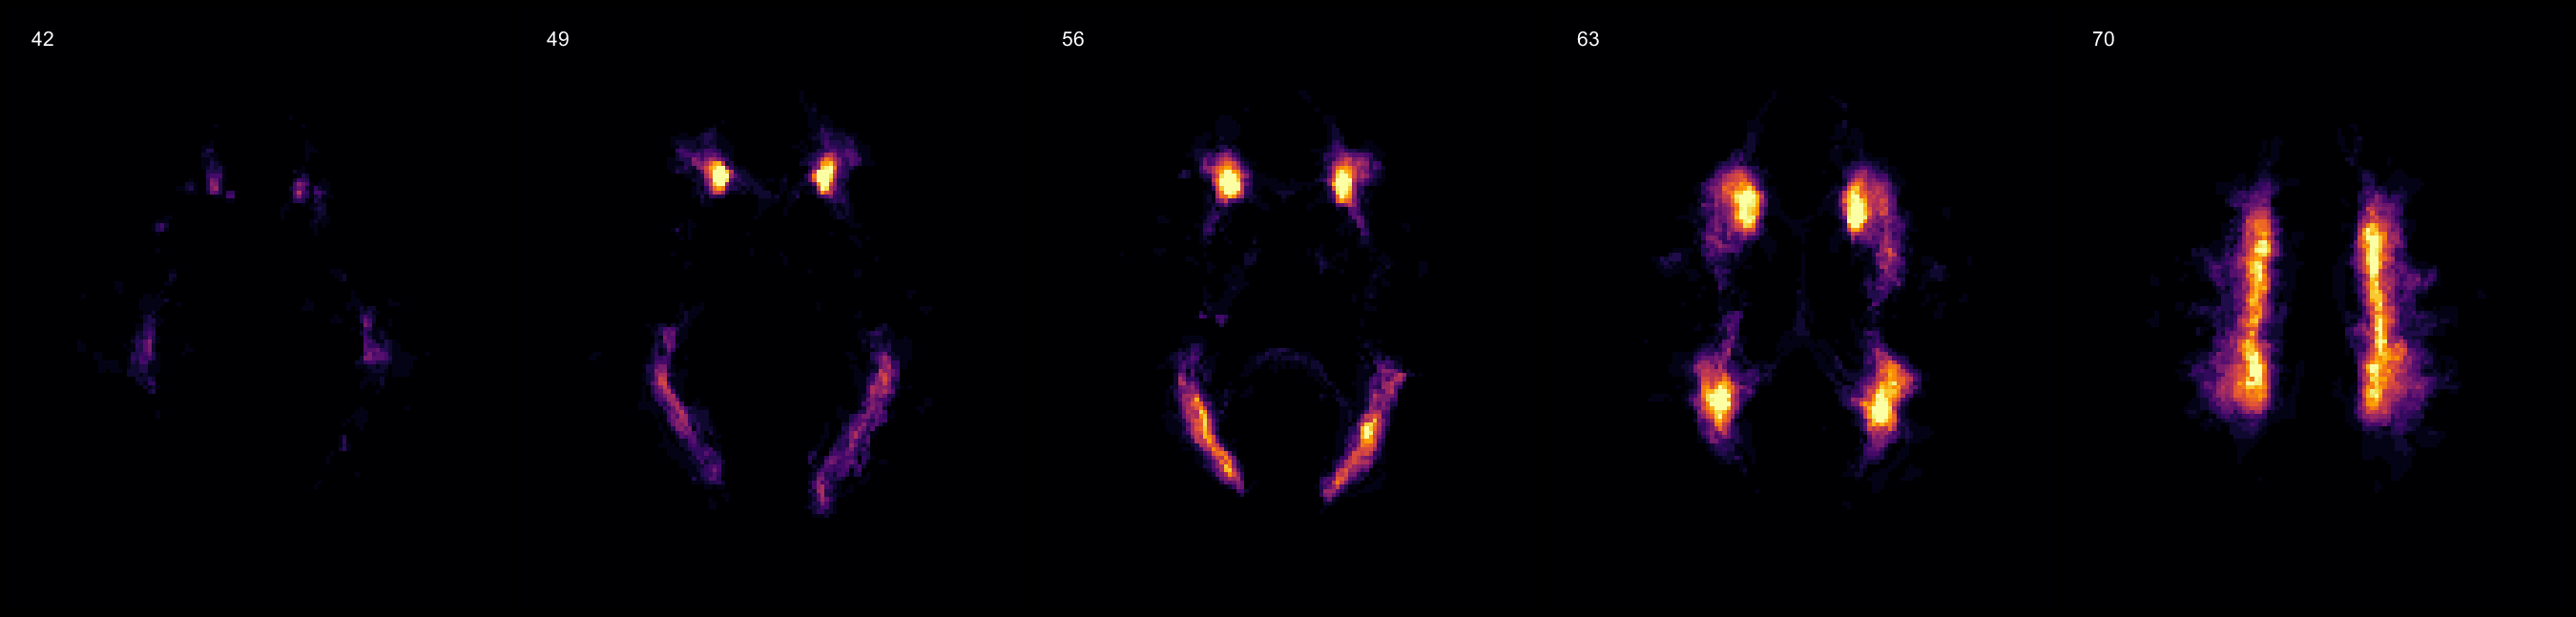
\includegraphics[height=\sliceheight]{rawthropt-tp.png} 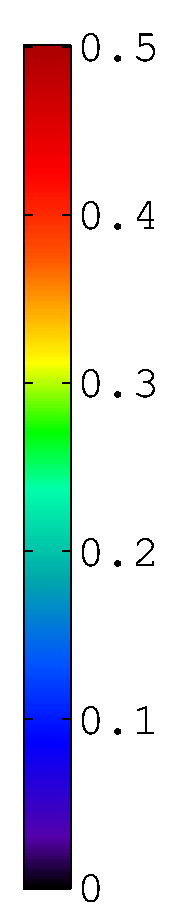
\includegraphics[height=\sliceheight]{cbar-NIH3-0-05}\end{subfigureside}\\[0.5em]
%    \begin{subfigureside}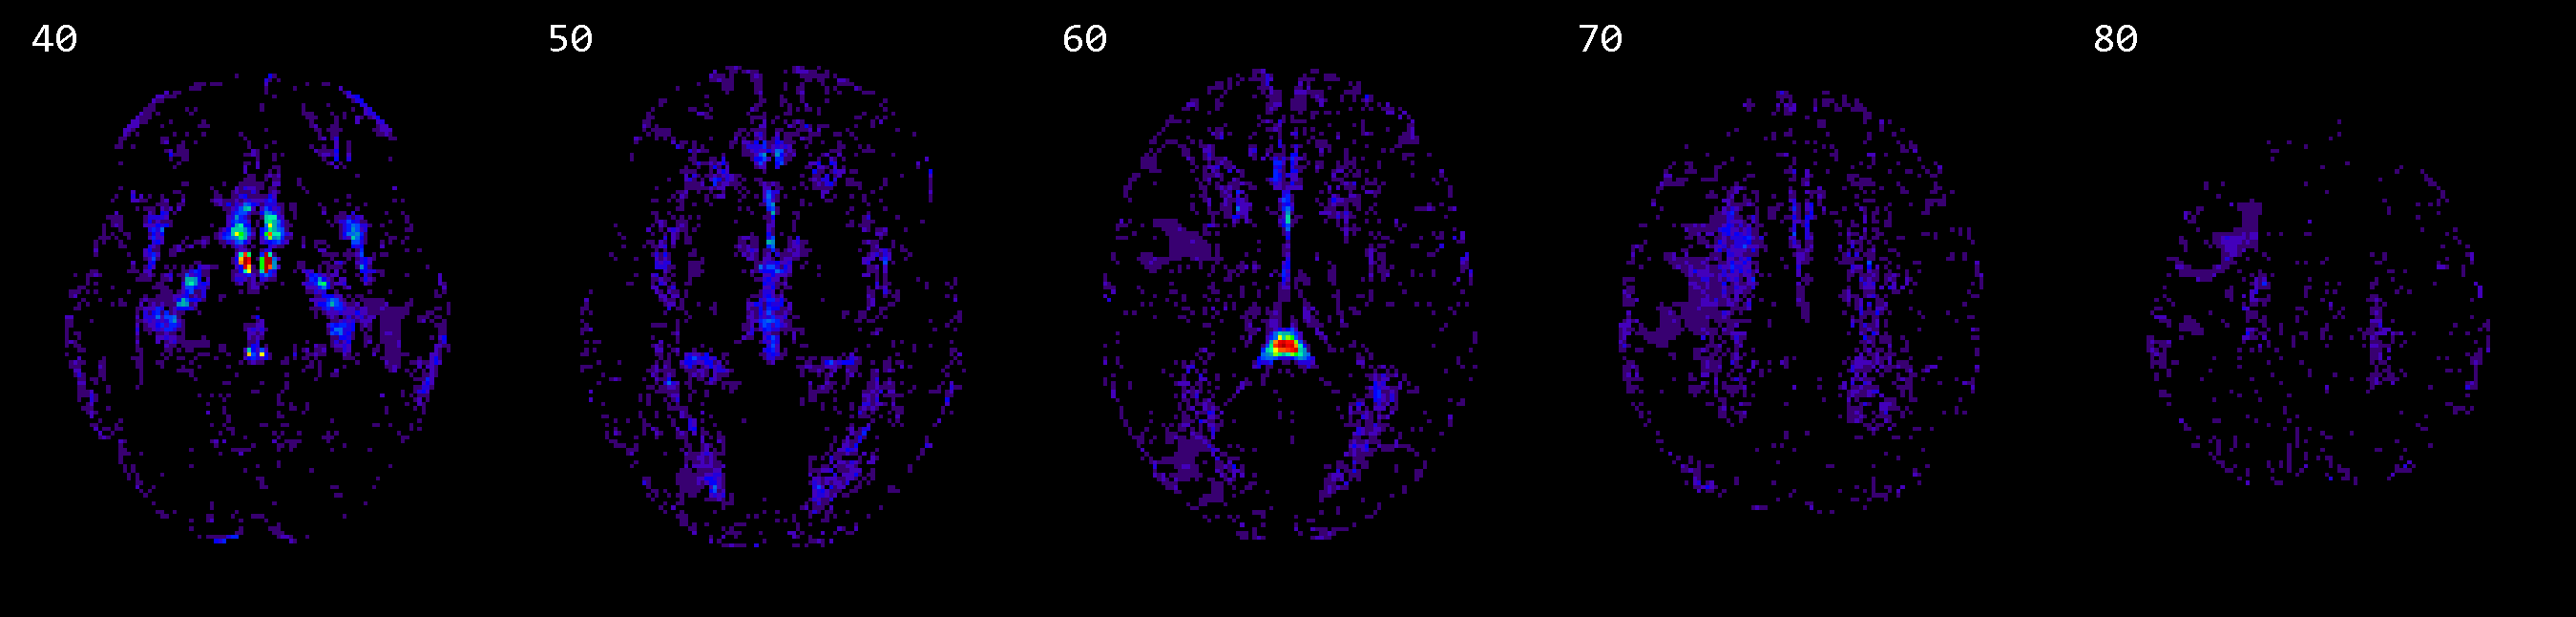
\includegraphics[height=\sliceheight]{rawthropt-fp.png} 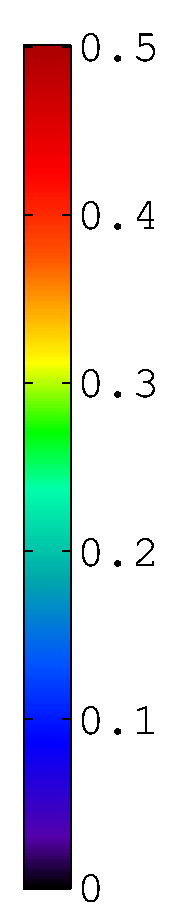
\includegraphics[height=\sliceheight]{cbar-NIH3-0-05}\end{subfigureside}\\[0.5em]
%    \begin{subfigureside}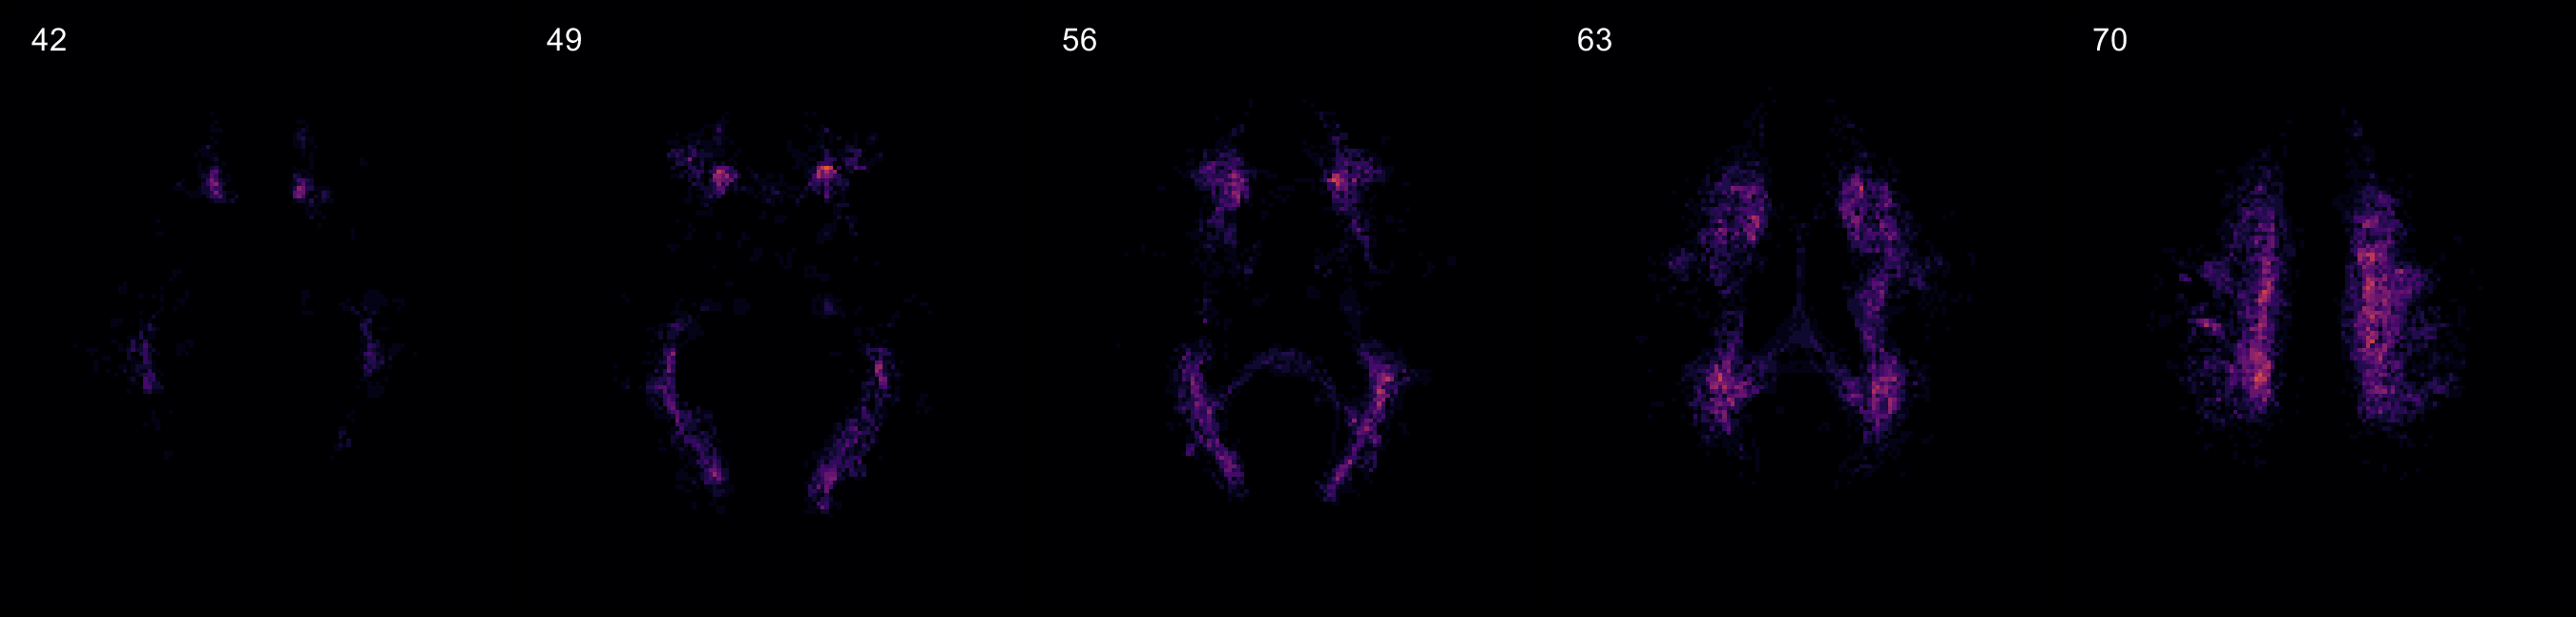
\includegraphics[height=\sliceheight]{rawthropt-fn.png} 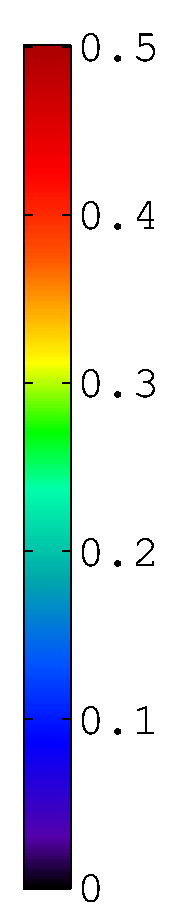
\includegraphics[height=\sliceheight]{cbar-NIH3-0-05}\end{subfigureside}\\[0.5em]
%    \caption{}
%  \end{figure}
%\begin{figure}\centering
%  \begin{minipage}{6cm}
%    \begin{subfigure}{\textwidth}
%      \centering\subcaption{Original}\label{fig:m08-rev-o}
%      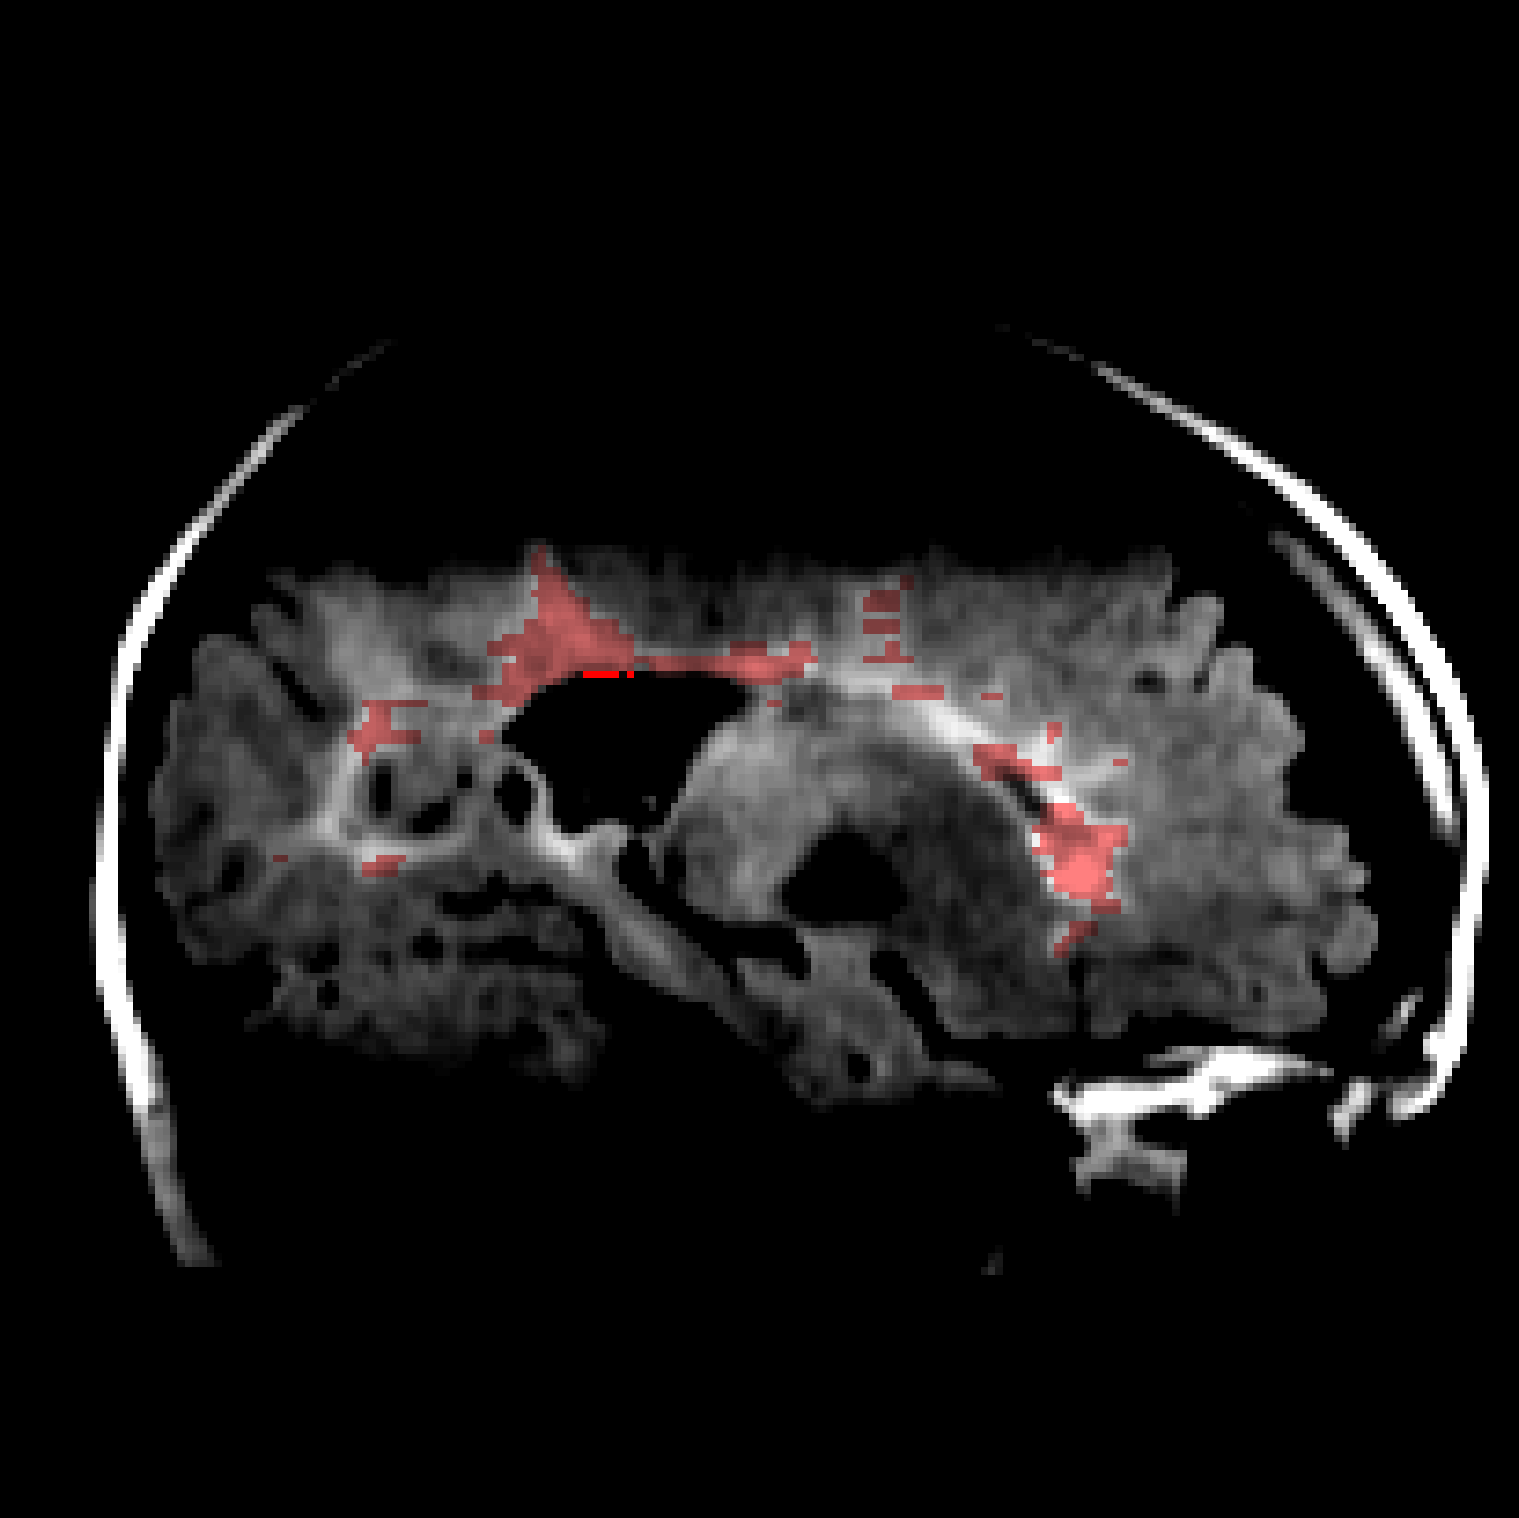
\includegraphics[height=6cm]{m08rev-01-d2-z146-o}\\[0.2em]
%      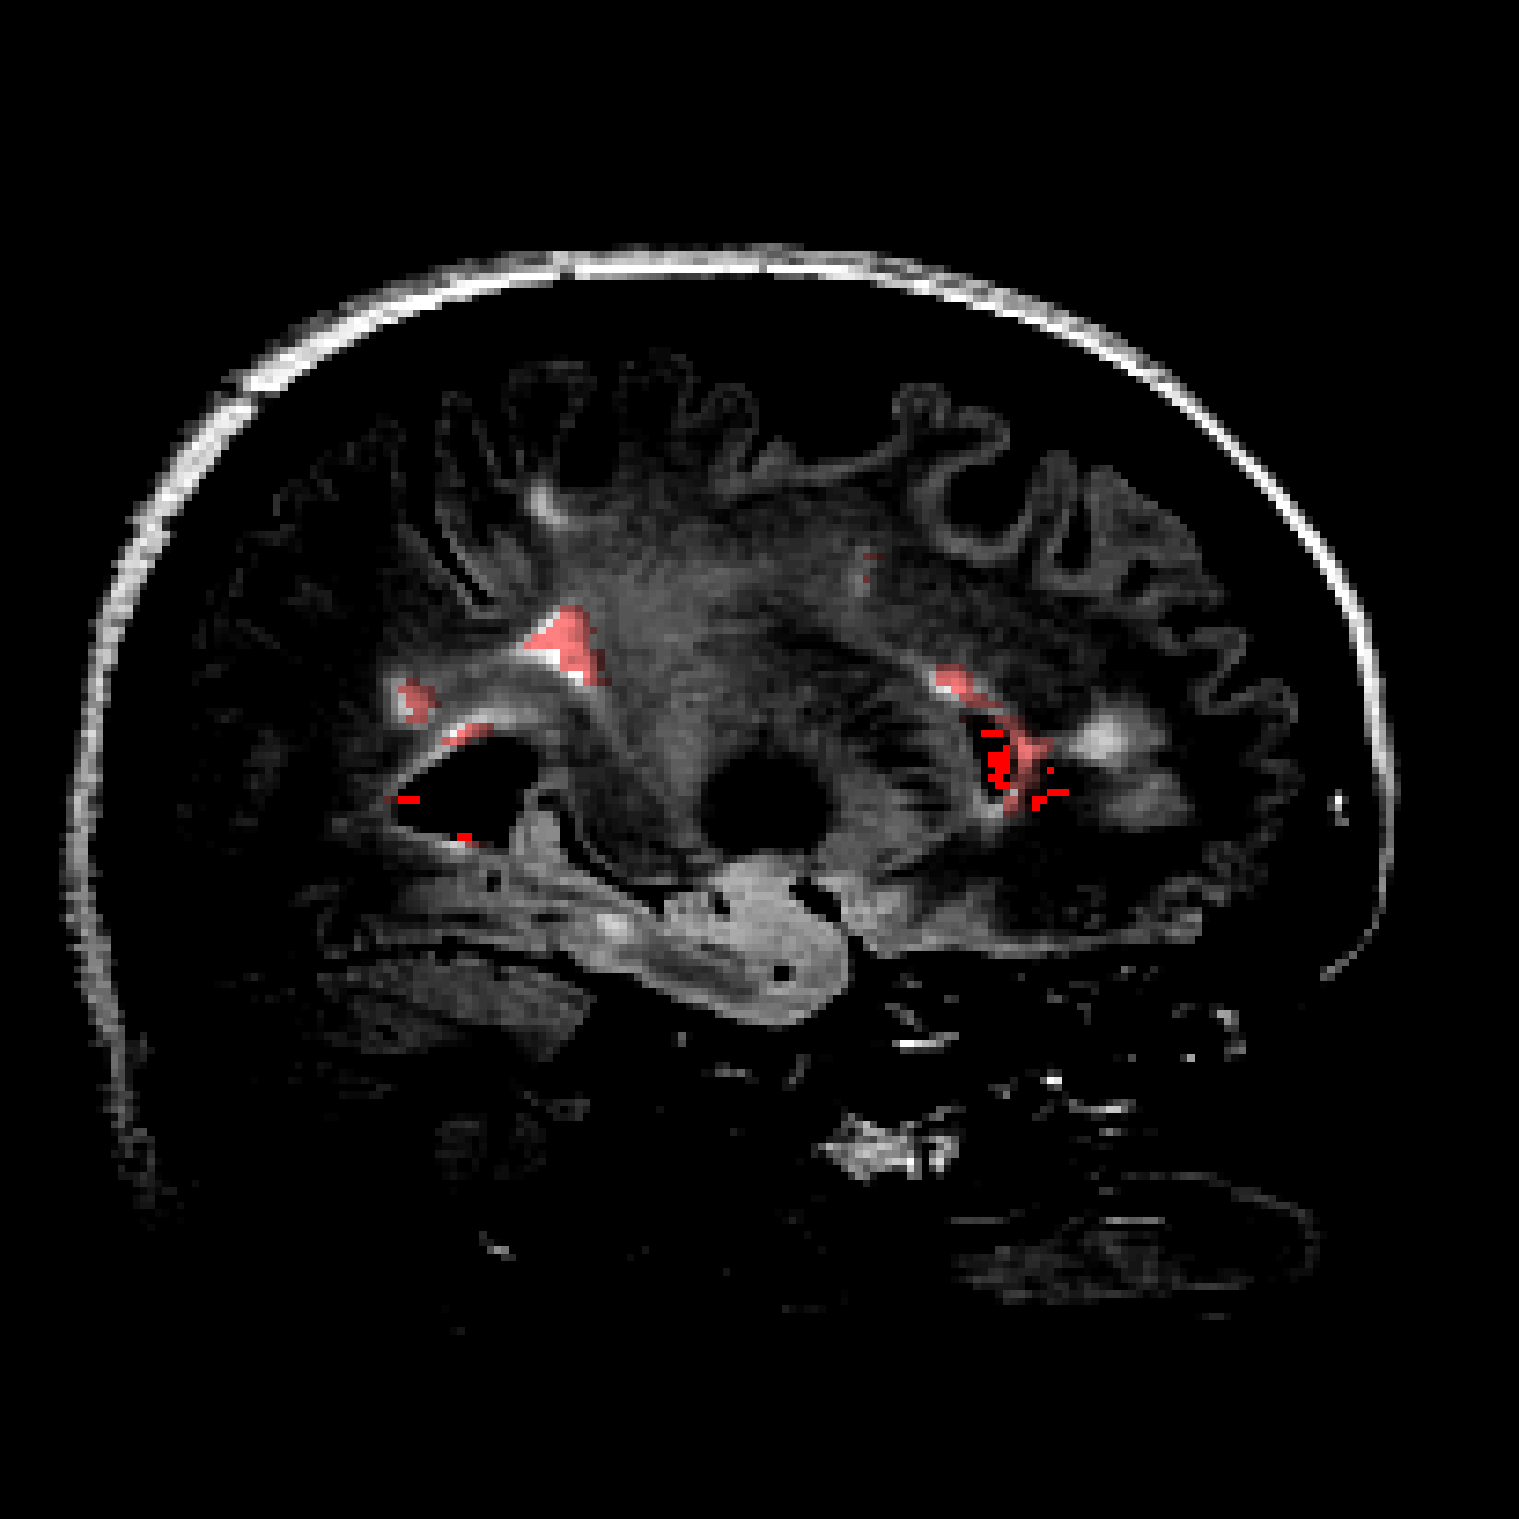
\includegraphics[height=6cm]{m08rev-05-d2-z107-o}\\[0.2em]
%      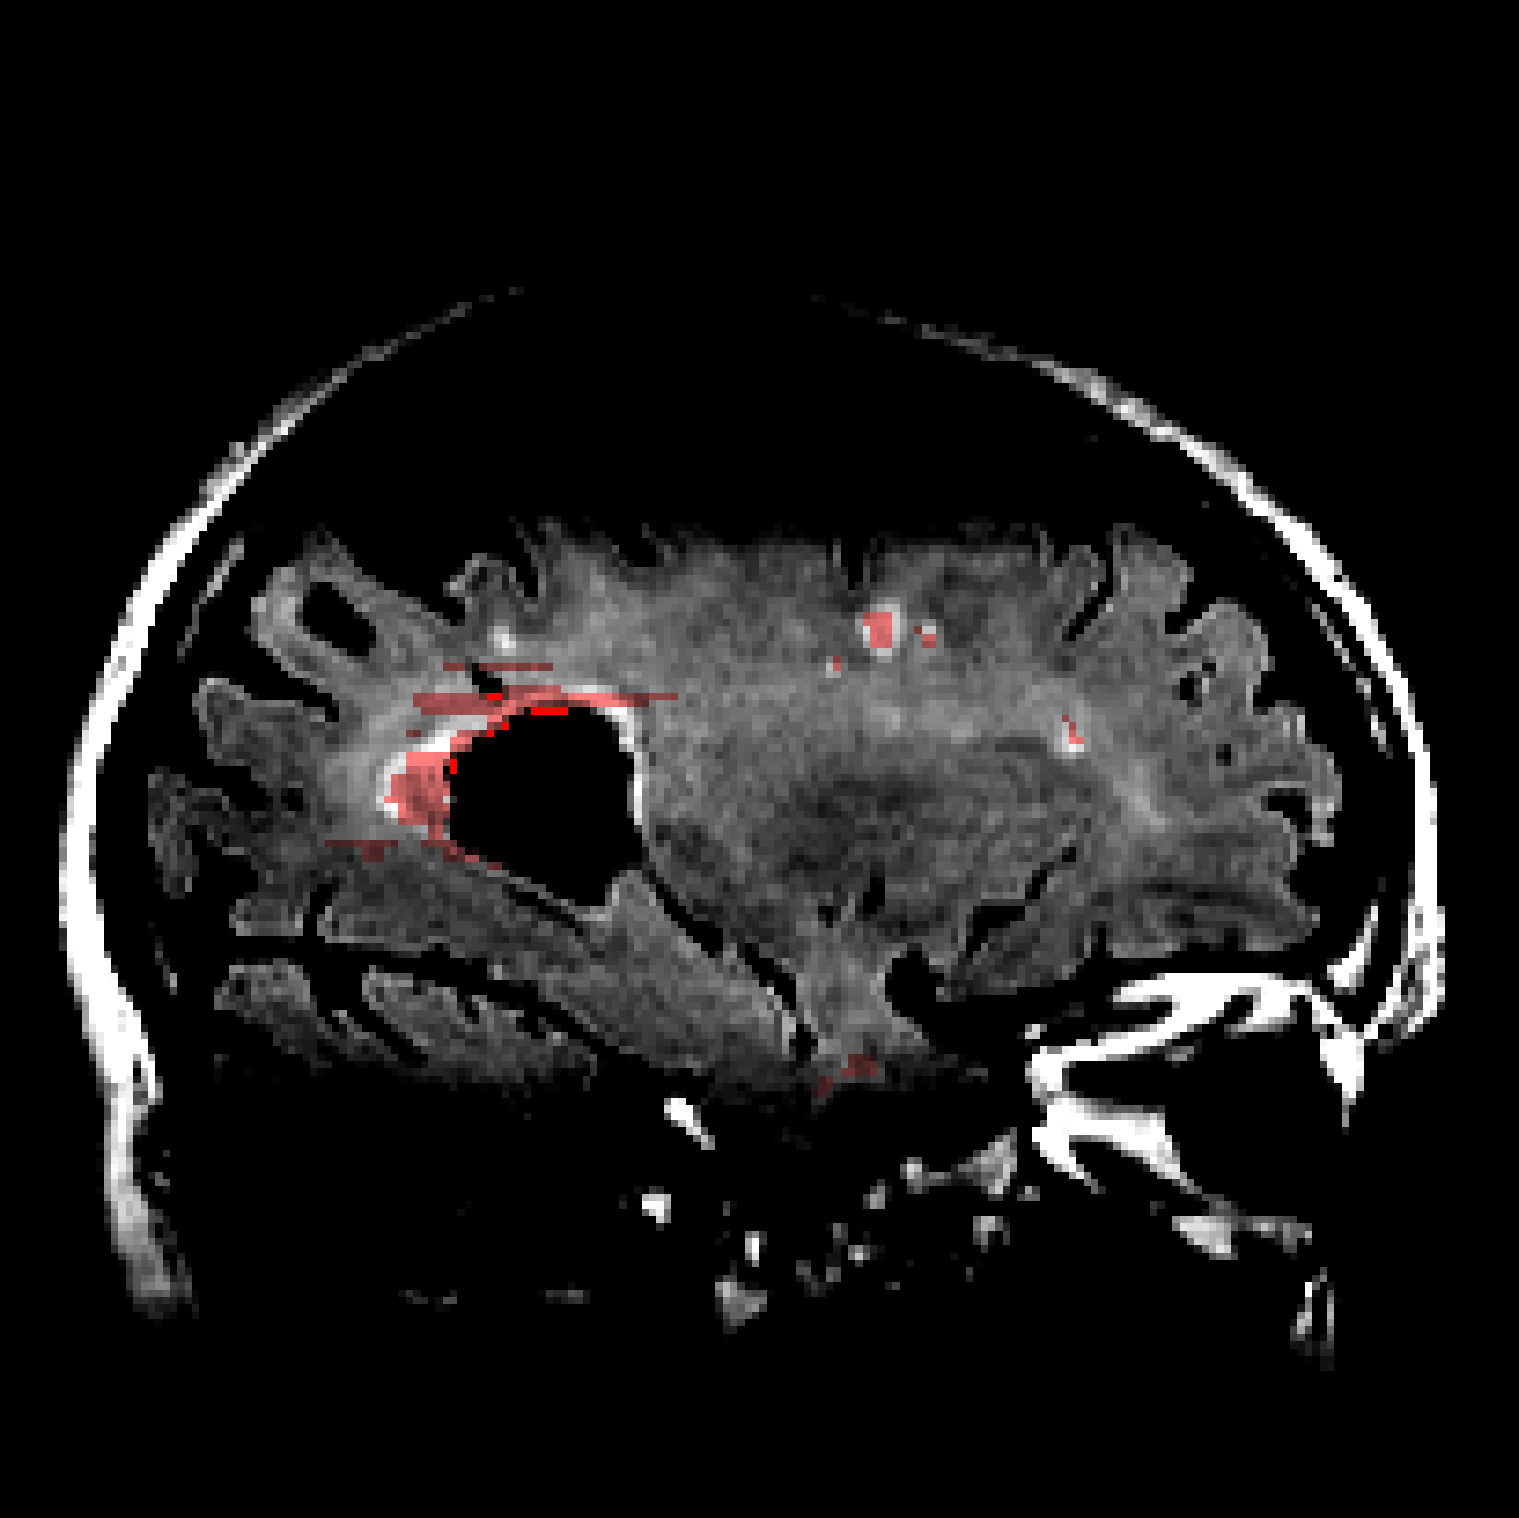
\includegraphics[height=6cm]{m08rev-06-d2-z101-o}
%    \end{subfigure}
%  \end{minipage}
%  \begin{minipage}{6cm}
%    \begin{subfigure}{\textwidth}
%      \centering\subcaption{Revision}\label{fig:m08-rev-r}
%      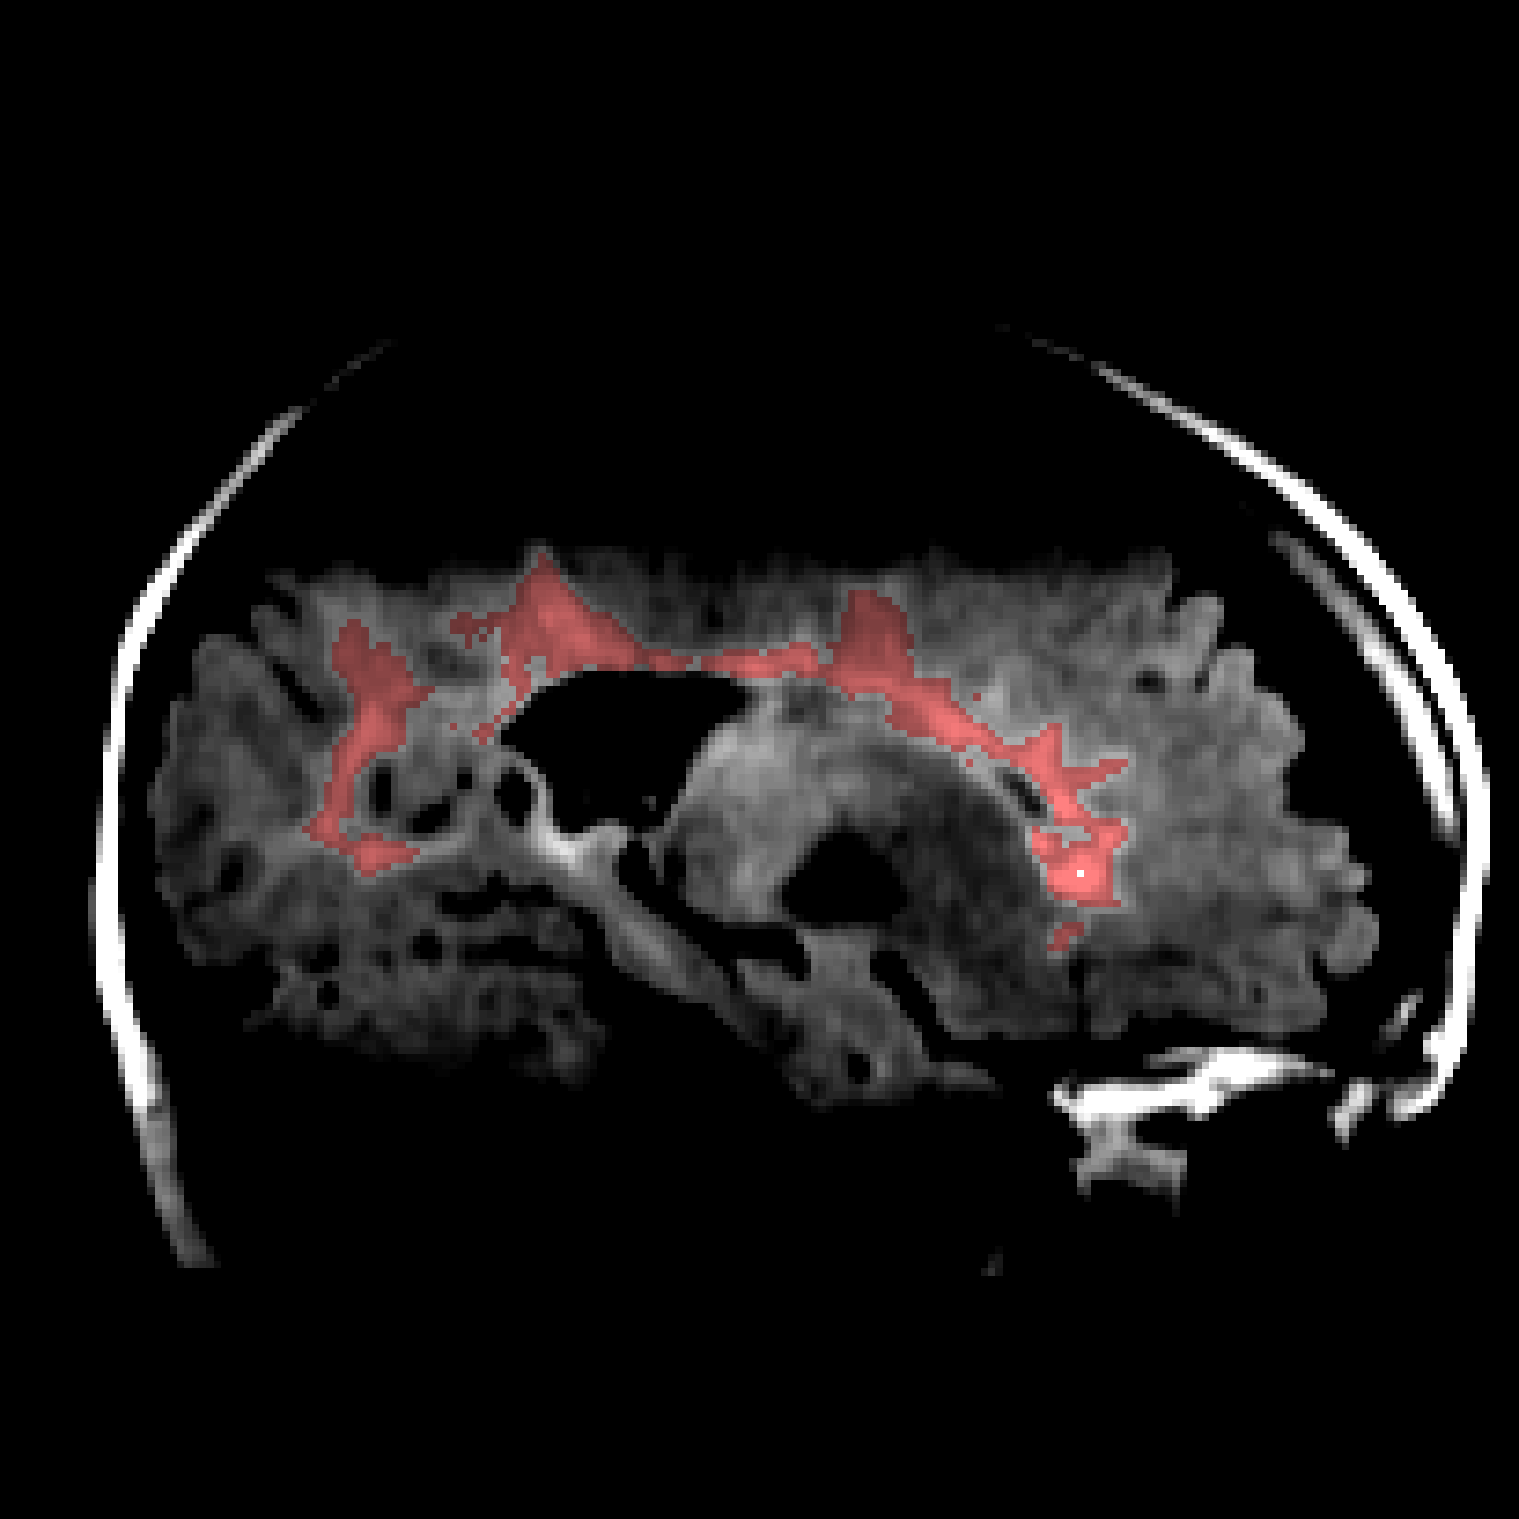
\includegraphics[height=6cm]{m08rev-01-d2-z146-r}\makebox[0pt][r]{\textcolor{white}{ CHB 01 }}\\[0.2em]
%      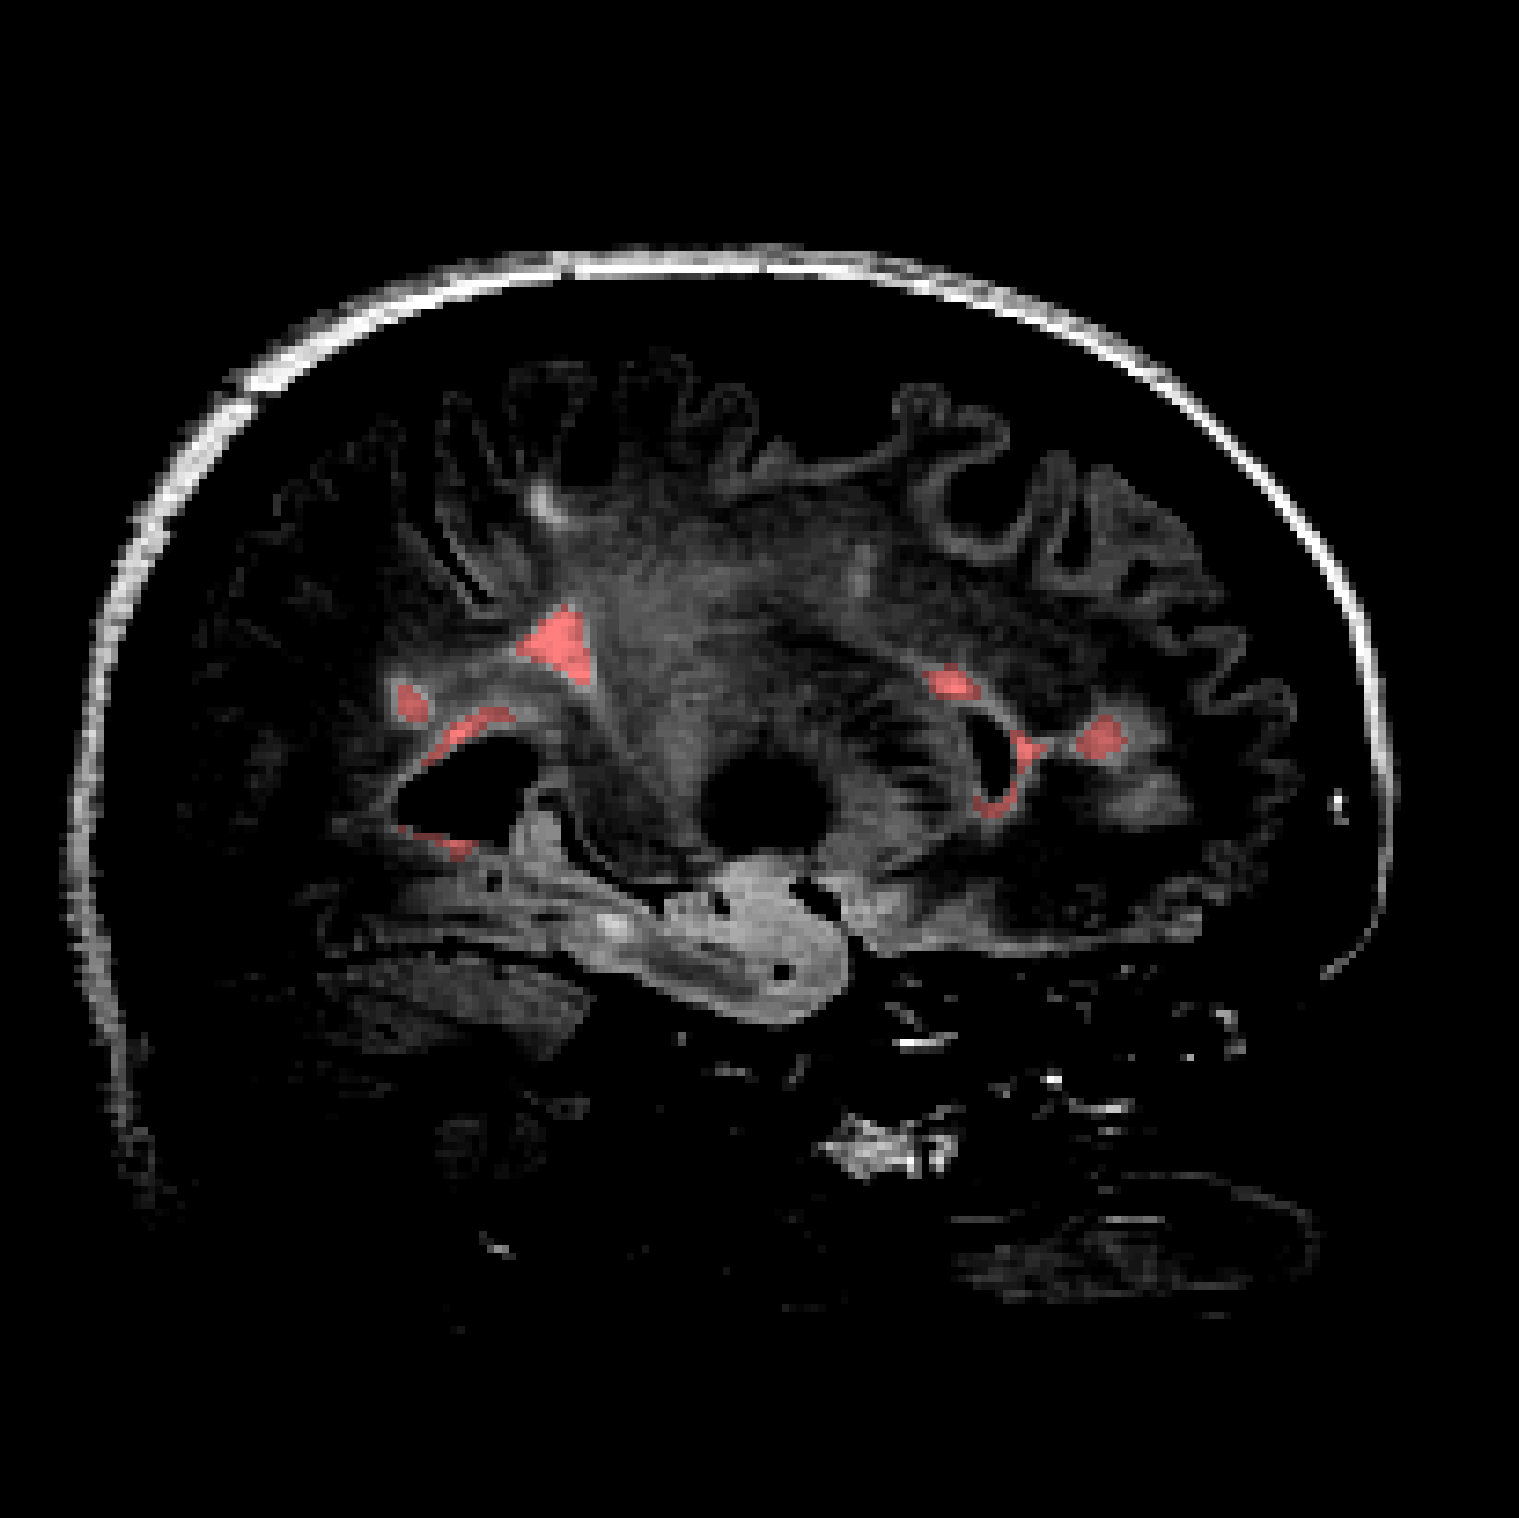
\includegraphics[height=6cm]{m08rev-05-d2-z107-r}\makebox[0pt][r]{\textcolor{white}{ CHB 05 }}\\[0.2em]
%      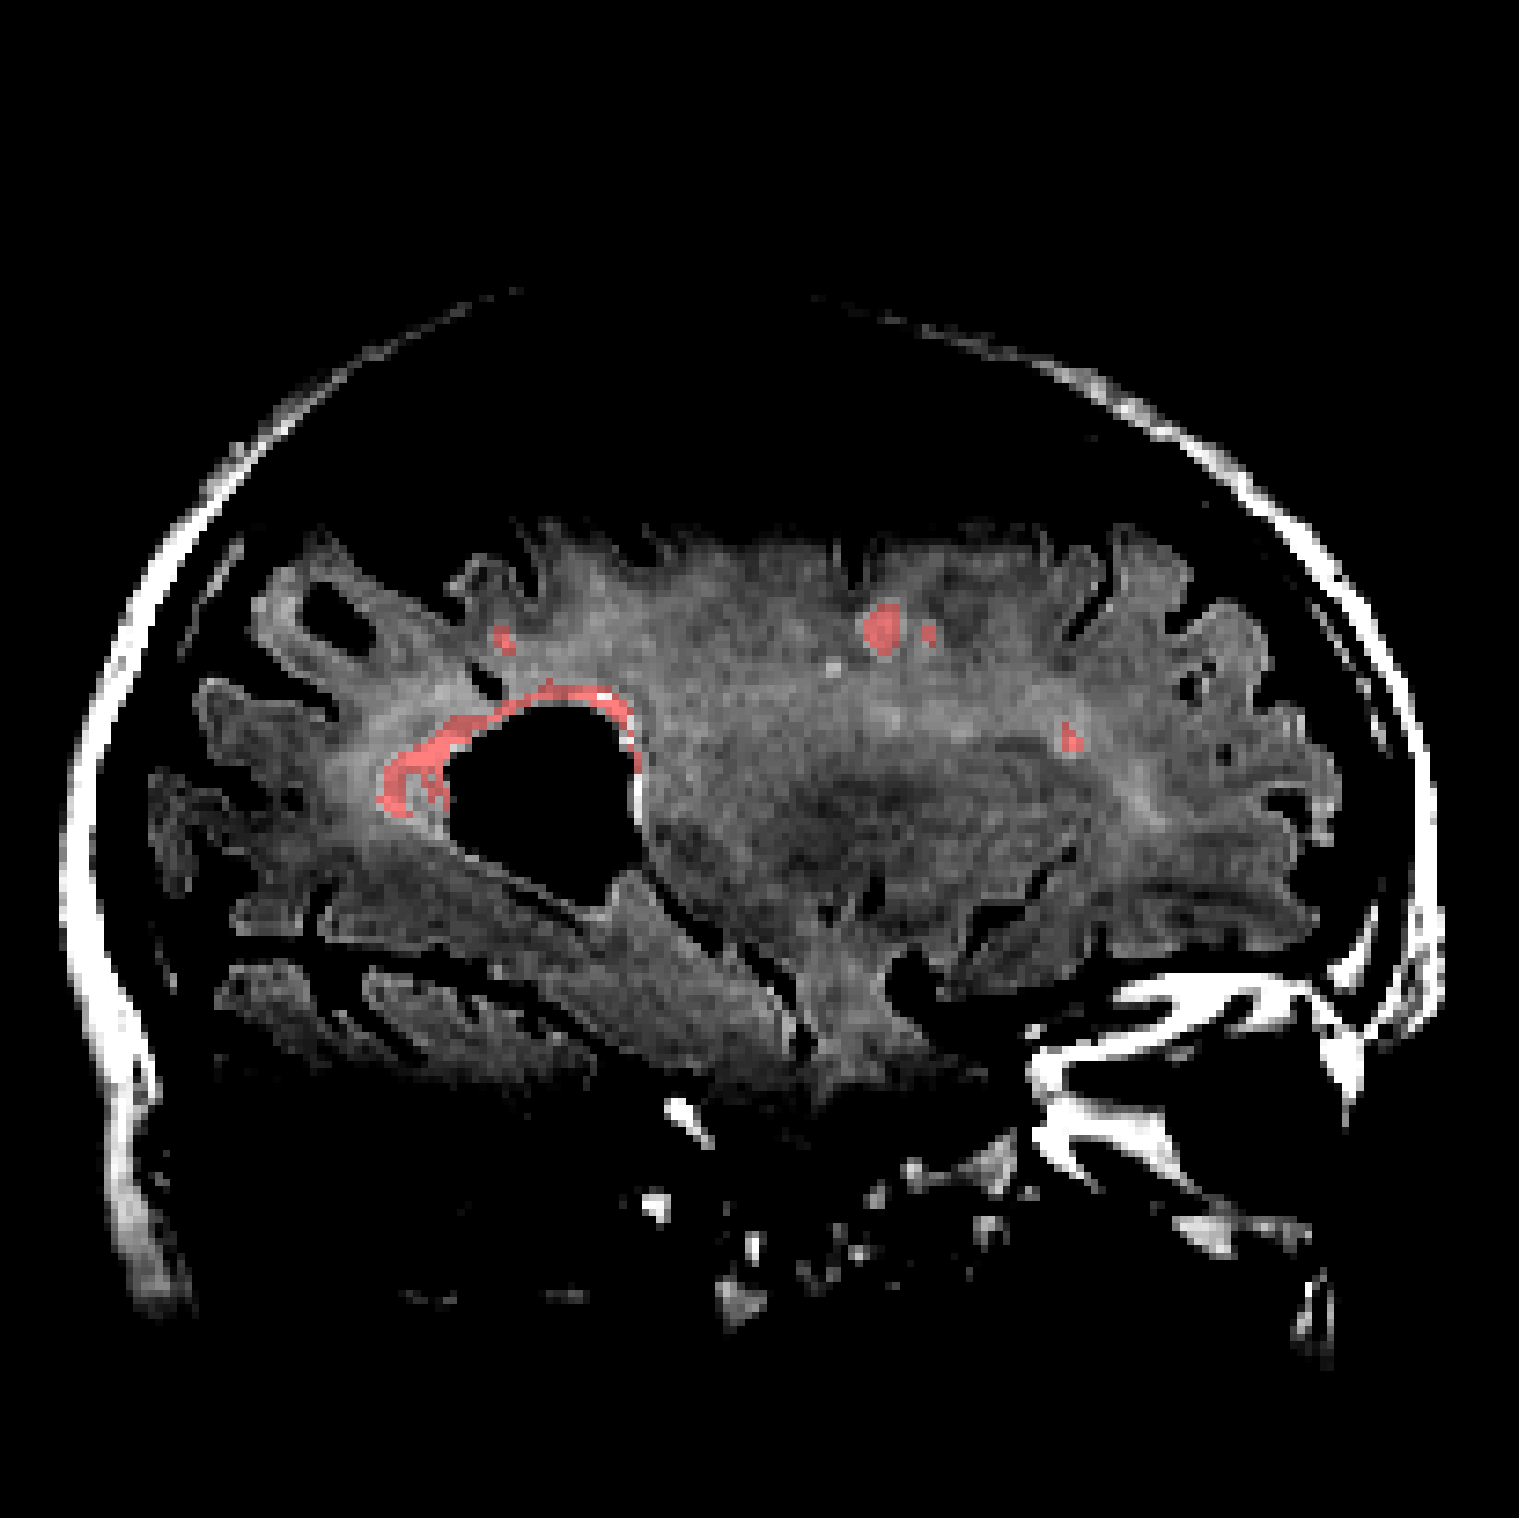
\includegraphics[height=6cm]{m08rev-06-d2-z101-r}\makebox[0pt][r]{\textcolor{white}{ CHB 06 }}
%    \end{subfigure}
%  \end{minipage}
%\end{figure}
The VLR model draws inspiration for the LPA model by Schmidt2015 from the public toolbox LST; however, no publication is associated with this algorithm. An understanding of the main segmentation model was derived from the code, as shown here. Following various standardization steps, the probability of lesion (``\texttt{prob}'') is computed as
\begin{matlab}
% Linear predictor
eta = intercept + Bf2_eff .* Bf2(indx_brain) + sp_Bf2(indx_brain);
% ...
% Probabilities
prob(indx_brain) = 1 ./ (1+ exp(-eta));
\end{matlab}
Mathematically, this can be written as
\begin{equation}
P(c(x)=1\mid y,\b_0,\b_y,\b_x) = \frac{1}{1+e^{-\eta(x)}},\qquad\eta(x) = \b_0 + \b_y y(x) + \b_x(x)
\end{equation}
\includecode{logreg.m}
\end{doublespace}
\end{document}